We conducted a brief benchmarking of the various studied techniques for adaptive and individualized DP-SGD, the purpose of which is two-fold: first, some of the experimental runs in the original papers introducing these techniques were conducted under different datasets and/or different parameter settings, making it difficult to directly compare approaches head-to-head. Second, we wanted to validate the results presented by the authors in their papers, and thus conduct a reproducibility study. 
%We are going to include comparative findings from experiments for the various suggested methodologies in this section. In addition to examining the impact of the recently emerging research trend of Privacy Budget Individualization covered in section \ref{sec:individ}, we experiment traditional DPSGD with several parameters adaptation approaches from those that were covered in section \ref{sec:adaptation}. 
For all experiments, we use the RDP moments accountant as defined by Abadi et. al. in~\cite{RefWorks:RefID:40-abadi2016deep}, based on the concept of Renyi Differential Privacy discussed in Section~\ref{bckg}.

We used two prominent datasets in our runs:
\begin{itemize}
    \item MNIST: introduced by LeCun et al.~ \cite{mnist} in 1998, consists of handwritten digit images. Specifically, it contains 60,000 training examples and 10,000 test examples, where each example is a 28×28 grayscale image.
    \item CIFAR-10: Developed by Krizhevsky and Hinton in 2009~\cite{cifar}, it consists of color images classified into ten distinct classes, including objects like airplanes, cars, and birds. It includes 50,000 training images and 10,000 test images, with each image being a 32×32 pixel RGB image.
\end{itemize}

\subsection{Adaptive DP-SGD Results}
First, we investigated three prominent techniques for noise magnitude decaying discussed in Section~\ref{decay}: Time Decay, Exponential Decay and Polynomial Decay \cite{RefWorks:RefID:47-yu2019differentially}. These experiments were performed using the same parameters settings as in the original work from~\ref{decay} ($\sigma_{initial} = 10$  for all decaying strategies) on the MNIST dataset. Figure~\ref{decayRate} and Table~\ref{tab: decayAcc} summarize the results. Our experiments show that these techniques assign very low privacy budget ($\epsilon$) to the earlier iterations with a controlled increase over time, allowing the training gradients to be injected with higher noise at the start of training, and reducing the noise in later iterations, as training converges. Figure~\ref{decayRate} illustrates the privacy budget consumption rate for all mentioned techniques along with standard DP-SGD for $\sigma_{fixed}=8$. Among all approaches, Time Decay consumes the most privacy-budget, and at the highest rate. Table~\ref{tab: decayAcc} presents the testing accuracy achieved using the above-mentioned decaying strategies. Time Decay achieves the highest accuracy of $91.50$\% after consuming approximately $\epsilon = 1.0$ while Polynomial Decay and Exponential Decay achieved $90.66$\% and $89.00$\% respectively, for the same aggregate privacy budget consumption.

\begin{table}[!htp]\centering
\caption{Accuracy Comparison of Noise Decay Strategies}\label{tab: decayAcc}
\scriptsize
\begin{tabular}{|p{1.7cm}|p{1.7cm}|p{1.7cm}|r|p{1.7cm}|p{1.7cm}|}\toprule
\hline
\textbf{Stopping Criterion} &\textbf{Stopping Threshold} &\textbf{Polynomial Decay} &\textbf{Time Decay} &\textbf{Exponential Decay}  \\\midrule
\hline
Epochs &100 &$91.67$\% &$92.18$\% &$87.41$\% \\
\hline
\large $\epsilon$ &1 &$90.66$\% &$91.50$\% &$89.00$\% \\
\hline
\bottomrule
\end{tabular}
\end{table}

\begin{figure}[h]
\centering
        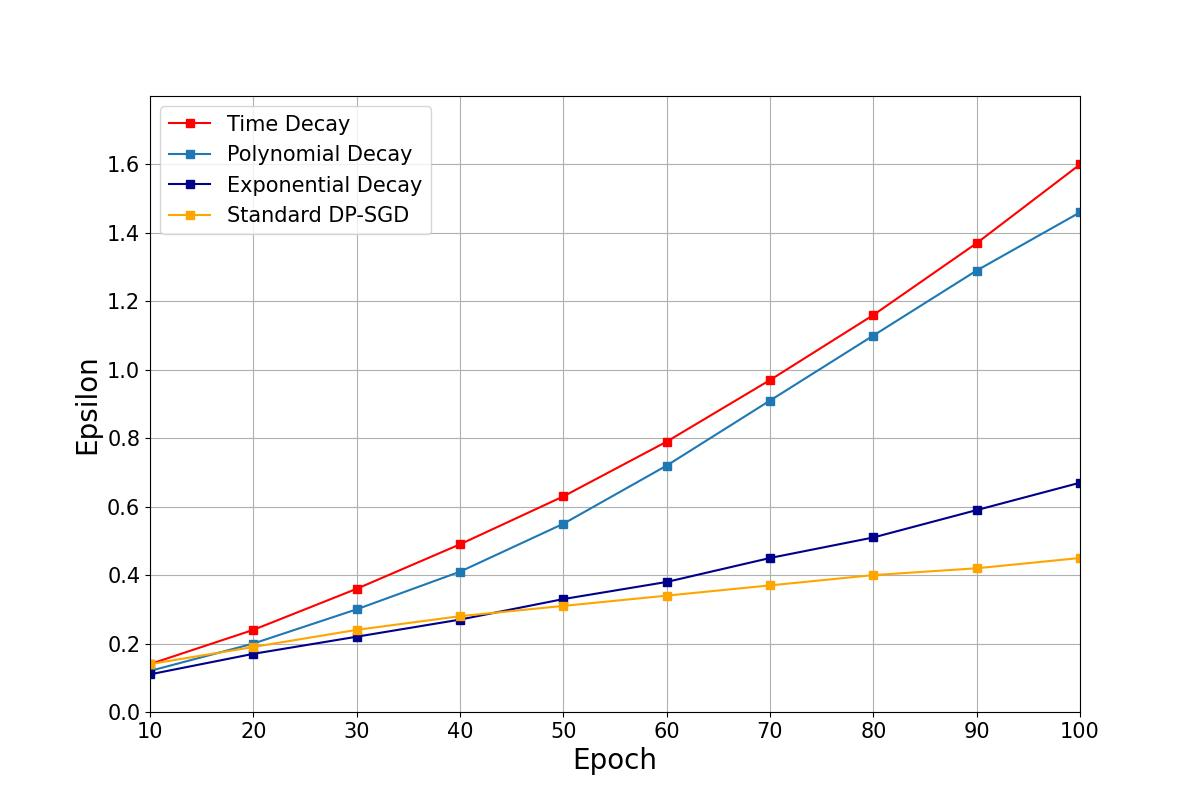
\includegraphics[width=0.7\linewidth]{submissions/submission5/figs/epsDecay.jpg}
   \caption{Adaptive Privacy Budget Consumption Rate}\label{FigDiff}
   \label{decayRate}
\end{figure} 

Next, we experimented with adapting learning rate ($\eta$) and clipping threshold ($C$), according to the methodology described in~\cite{RefWorks:RefID:38-koskelalearning} and~\cite{RefWorks:RefID:37-andrewdifferentially} (described in Sections~\ref{sec:quantile} and~\ref{sec:lr}, respectively). Noise magnitude was set at $\sigma=2.0$. 
Figure~\ref{accadapt} shows the test accuracy of each technique when training on the MNIST dataset. 
Among the three, adaptive learning rate produced the best accuracy ($91.90$\%) after consuming privacy budget $\epsilon=1.0$, while adaptive clipping achieved $85.37\%$ accuracy with overall privacy budget consumption of $\epsilon=0.83$ -- a tighter privacy guarantee than standard DP-SGD which achieved accuracy of $86.00$\% after consuming $\epsilon=1.0$. 

For comparison purpose, we tested the performance of the noise magnitude time decay methodology discussed earlier using the same parameters that have been used for the latest adaptation experiments. The noise magnitude time decay seems to be the most promising among all, as it yielded an accuracy of $92.05$\% with $\epsilon = 1.0$ in a shorter training time. 
\begin{figure}[h]
\centering
        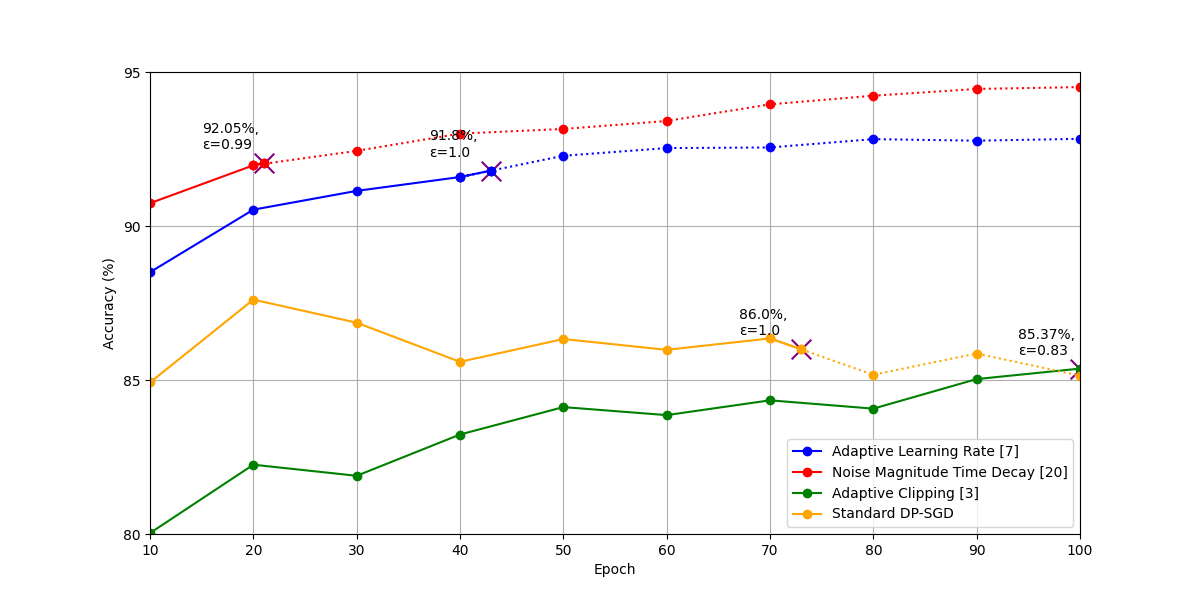
\includegraphics[width=\linewidth]{submissions/submission5/figs/AccAdapt.png}
   \caption{Accuracy of Adaptive Techniques on MNIST}
   \label{accadapt}
\end{figure} 

We conducted the same experiment on the CIFAR-10 dataset, using the same architecture and parameters used in~\cite{RefWorks:RefID:38-koskelalearning}, and $\sigma = 1.2$ for all techniques except for the exponential noise decaying approach, for which we used $\sigma_{initial} = 2.0$, in order to prevent very high privacy budget consumption. 
Figure~\ref{accadaptcifar} summarizes the results. 
Experiments on CIFAR-10 confirm the superiority of learning rate adaptation, which obtained the highest accuracy of $62.52\%$ with $\epsilon = 2.0$ going up to $64.97\%$ with $\epsilon = 3.0$. Clipping threshold adaptation produced slightly better improvements with an average of $7\%$ additional accuracy when compared to standard DP-SGD at similar privacy levels.
One important observation from this set of experiments is the performance of noise magnitude decay. Specifically, exponential noise decay is able to achieve only marginally better accuracy compared with the standard DP-SGD under similar budget consumption.

\begin{comment}
\begin{enumerate}
    \item Privacy budget consumption rate
    \item Performance improvement rate
    \item Rate of increase in the privacy budget consumption rate (resulted from the noise magnitude decay rate)
\end{enumerate}
\end{comment}

%Having a high rate of increase in the privacy budget consumption rate with a comparably high performance improvement rate can result in a better performance depending on the situation. What happened when we tried on MNIST with noise magnitude time decay is that there was a very high rate of privacy consumption but that was enough to have a higher performance improvement rate. On the other hand, CIFAR-10 is a more complicated and challenging dataset on which the performance increase is hard and need more detailed training, so what happened is that the performance improvement rate was not on the same level with the increase in the privacy budget consumption resulting in a drawback. So, in this case the choice of the noise magnitude adaptation strategy and the decay rate is very crucial along with a more powerful model architecture. In the original research \cite{RefWorks:RefID:47-yu2019differentially} they used VGG-16 architecture which reported a slight improvement with additional $2\%$ accuracy. Figure \ref{accadaptcifar} performance comparison along time on CIFAR-10 dataset



\begin{figure}[h]
\centering
        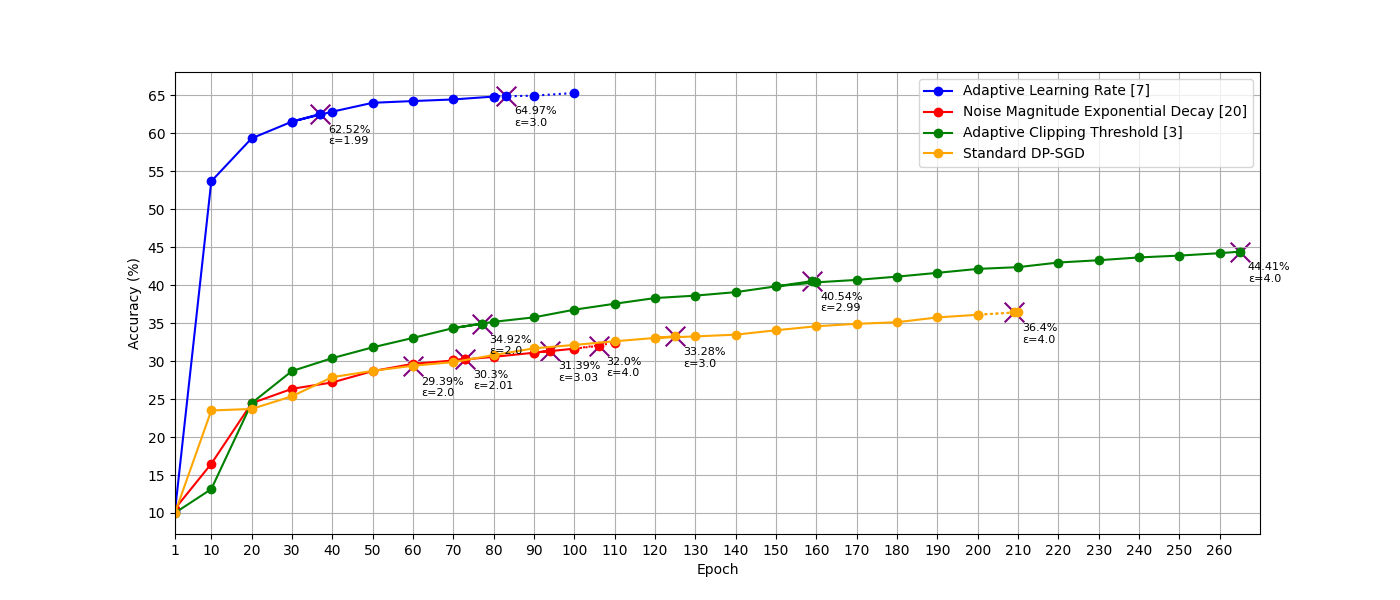
\includegraphics[width=\linewidth]{submissions/submission5/figs/AccAdaptCifar.png}
   \caption{Accuracy of Adaptive Techniques on CIFAR-10}
   \label{accadaptcifar}
\end{figure} 

\subsection{Individualized Privacy Budget Results}
We evaluate two different individualized privacy (IDP) approaches proposed by Boenisch et. al. in ~\cite{haveit}, namely {\em grouping} and {\em sampling}. We divide the training dataset into three partitions according to the privacy requirements illustrated in Table~\ref{tab: distrib}. The two distributions correspond to the settings used in~\cite{haveit} and~\cite{haveit2}, respectively. 

%A data pre-processing step is performed to extract the individualization parameters before training the model. 
First we present results obtained on the MNIST dataset. 
%with the mentioned data distribution considering the privacy budgets of Case 1 in table \ref{tab: distrib}. In our experiments, 
According to~\cite{haveit}, the sampling approach uses individual sampling rates = \{0.005, 0.009, 0.013\} for the three different privacy level groups respectively, with $\sigma_{sample}=1.368$. In the scaling approach, the corresponding individual clipping thresholds are \{0.141, 0.236, 0.299\} with $\sigma_{scale}=1.545$. After training the model using both approaches, scaling obtained accuracy of $97.63$\% while sampling achieved $96.79$\% accuracy, both outperforming previously mentioned DP-SGD related approach. The results match the ones presented in the original IDP work from~\cite{haveit}.

We also investigated results on CIFAR-10, which were not reported previously. We include two more extreme cases of privacy requirements, cases 2 and 3 in Table~\ref{tab: distrib}. Case 1 is the only one used in the original work from~\cite{haveit}. The second case has a more pronounced variability in privacy concerns, with one group having very tight privacy requirements, while the others are more loose. Finally, the third case has two groups with relatively tight privacy requirements, and a third with almost no privacy concerns. 

Figures~\ref{sampleEps} and~\ref{scaleEps} show the privacy consumption rates for each group in case 1. As shown in Figure~\ref{accidpcifar} and Table~\ref{tab: accIDP}, both grouping and sampling approaches were able to deal with the extreme cases, with the scaling approach giving better performance in cases 2 and 3. The most extreme cases lead to slowest convergence in training. This is a result of overfitting, as the sampled examples originate mostly in group 3, and thus the model finds it difficult to generalize results to less seen examples in groups 1 and 2. 

\begin{table}[!htp]\centering
\caption{Individualized Data Distributions}\label{tab: distrib}
\scriptsize
\begin{tabular}{|p{1.7cm}|p{1.7cm}|p{1.7cm}|p{1.7cm}|p{1.7cm}|}\toprule
\hline
\textbf{Group \#} &\textbf{Percentage of Data} &\textbf{Case 1}&\textbf{Case 2}&\textbf{Case 3}\\\midrule
\hline
\textbf{Group 1 (High Privacy)} &34\% &$\epsilon = 1.0$ &$\epsilon = 1.0$&$\epsilon = 1.0$\\
\hline
\textbf{Group 2 (Medium Privacy)} &43\% &$\epsilon = 2.0$&$\epsilon = 10.0$&$\epsilon = 2.0$ \\
\hline
\textbf{Group 3 (Low Privacy)} &23\% &$\epsilon = 3.0$ &$\epsilon = 20.0$&$\epsilon = 20.0$\\
\hline
\bottomrule
\end{tabular}
\end{table}


\begin{figure}[htbp]
  \centering
  \begin{minipage}[b]{0.45\textwidth}
   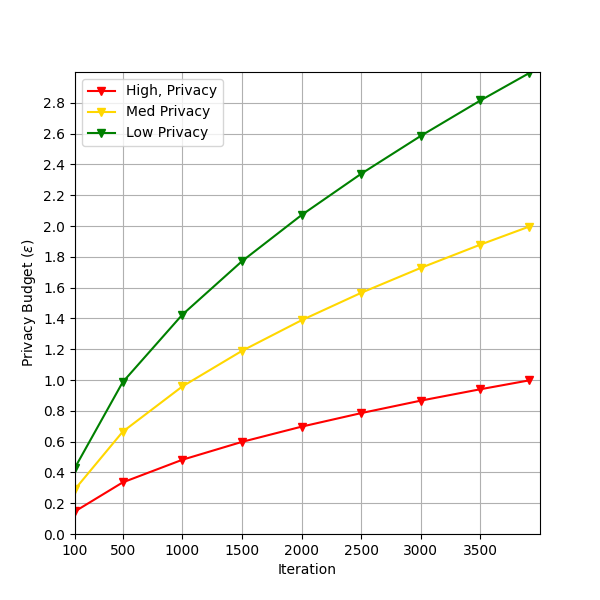
\includegraphics[width=\linewidth]{submissions/submission5/figs/epsindividone.png}
   \caption{Individualized privacy budget consumption over time (Sampling)}\label{FigDiff}
   \label{sampleEps}
  \end{minipage}
  \hfill
  \begin{minipage}[b]{0.45\textwidth}
    \centering
    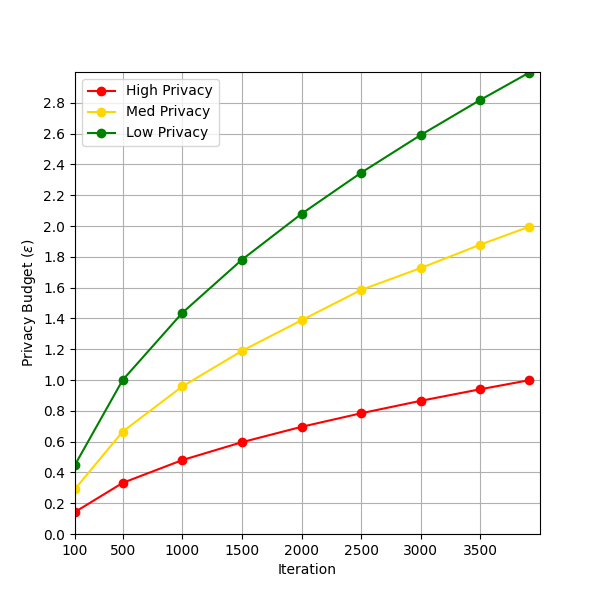
\includegraphics[width=\linewidth]{submissions/submission5/figs/epsindivid2.png}
   \caption{Individualized privacy budget consumption over time (Scaling)}\label{FigDiff}
   \label{scaleEps}
  \end{minipage}
  
\end{figure}

\begin{table}[!htp]\centering
\caption{Performance of IDP-SGD on CIFAR-10}\label{tab: accIDP}
\scriptsize
\begin{tabular}{|p{1.7cm}|p{1.7cm}|p{1.7cm}|p{1.7cm}|p{1.7cm}|}\toprule
\hline
\textbf{Approach}  &\textbf{Case 1}&\textbf{Case 2}&\textbf{Case 3}\\\midrule
\hline
\textbf{Sampling}  & 59.03\% & 59.49\% & 59.7\% \\
\hline
\textbf{Scaling} & 58.26\% & 67.64\% & 63.07\% \\
\hline
\bottomrule
\end{tabular}
\end{table}
\begin{figure}[h]
\centering
        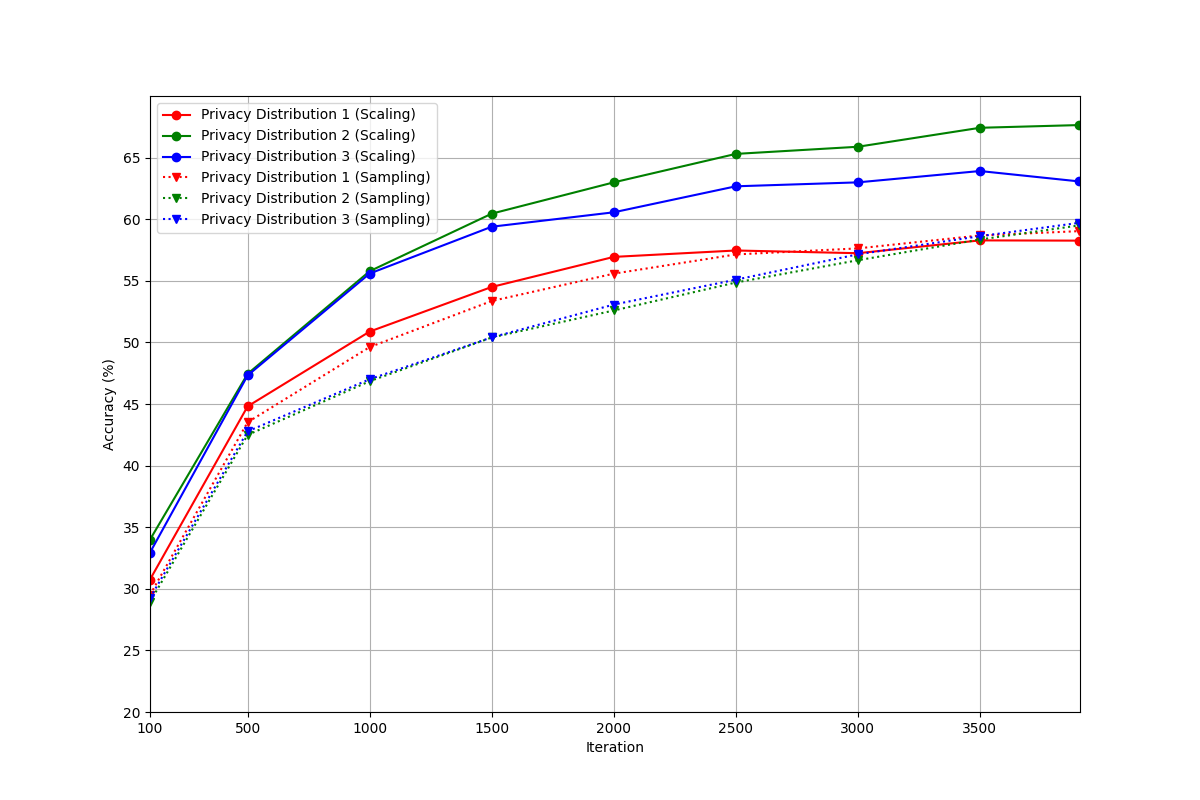
\includegraphics[width=\linewidth]{submissions/submission5/figs/cifarindivid.png}
   \caption{Testing accuracy for IDP-SGD techniques on CIFAR-10}\label{FigDiff}
   \label{accidpcifar}
\end{figure} 